%% abtex2-modelo-relatorio-tecnico.tex, v<VERSION> laurocesar
%% Copyright 2012-<COPYRIGHT_YEAR> by abnTeX2 group at http://www.abntex.net.br/
%%
%% This work may be distributed and/or modified under the
%% conditions of the LaTeX Project Public License, either version 1.3
%% of this license or (at your option) any later version.
%% The latest version of this license is in
%%   http://www.latex-project.org/lppl.txt
%% and version 1.3 or later is part of all distributions of LaTeX
%% version 2005/12/01 or later.
%%
%% This work has the LPPL maintenance status `maintained'.
%%
%% The Current Maintainer of this work is the abnTeX2 team, led
%% by Lauro César Araujo. Further information are available on
%% http://www.abntex.net.br/
%%
%% This work consists of the files abntex2-modelo-relatorio-tecnico.tex,
%% abntex2-modelo-include-comandos and abntex2-modelo-references.bib
%%

% ------------------------------------------------------------------------
% ------------------------------------------------------------------------
% abnTeX2: Modelo de Relatório Técnico/Acadêmico em conformidade com
% ABNT NBR 10719:2015 Informação e documentação - Relatório técnico e/ou
% científico - Apresentação
% ------------------------------------------------------------------------
% ------------------------------------------------------------------------

\documentclass[
	% -- opções da classe memoir --
	12pt,				% tamanho da fonte
	openright,			% capítulos começam em pág ímpar (insere página vazia caso preciso)
	twoside,			% para impressão em recto e verso. Oposto a oneside
	a4paper,			% tamanho do papel.
	% -- opções da classe abntex2 --
	%chapter=TITLE,		% títulos de capítulos convertidos em letras maiúsculas
	%section=TITLE,		% títulos de seções convertidos em letras maiúsculas
	%subsection=TITLE,	% títulos de subseções convertidos em letras maiúsculas
	%subsubsection=TITLE,% títulos de subsubseções convertidos em letras maiúsculas
	% -- opções do pacote babel --
	english,			% idioma adicional para hifenização
	french,				% idioma adicional para hifenização
	spanish,			% idioma adicional para hifenização
	brazil,				% o último idioma é o principal do documento
	]{abntex2}


% ---
% PACOTES
% --- How do I remove blank pages coming between two chapters in Appendix?
%\documentclass[oneside]{book}

% ---
% Pacotes fundamentais
% ---
\usepackage{lmodern}			% Usa a fonte Latin Modern
\usepackage[T1]{fontenc}		% Selecao de codigos de fonte.
\usepackage[utf8]{inputenc}		% Codificacao do documento (conversão automática dos acentos)
\usepackage{indentfirst}		% Indenta o primeiro parágrafo de cada seção.
\usepackage{color}				% Controle das cores
\usepackage{graphicx}			% Inclusão de gráficos
\usepackage{microtype} 			% para melhorias de justificação
% ---
\usepackage{graphicx} % Required for including pictures
\graphicspath{{img/}} % Specifies the directory where pictures are stored
% ---
% Pacotes adicionais, usados no anexo do modelo de folha de identificação
% ---
\usepackage{multicol}
\usepackage{multirow}
% ---

% ---
% Pacotes adicionais, usados apenas no âmbito do Modelo Canônico do abnteX2
% ---
\usepackage{lipsum}				% para geração de dummy text
% ---

% ---
% Pacotes de citações
% ---
\usepackage[brazilian,hyperpageref]{backref}	 % Paginas com as citações na bibl
\usepackage[alf]{abntex2cite}	% Citações padrão ABNT
\usepackage{verbatim}
% ---
% CONFIGURAÇÕES DE PACOTES
% ---
\usepackage{afterpage}
\usepackage{emptypage}


% ---
% Configurações do pacote backref
% Usado sem a opção hyperpageref de backref
\renewcommand{\backrefpagesname}{Citado na(s) página(s):~}
% Texto padrão antes do número das páginas
\renewcommand{\backref}{}
% Define os textos da citação
\renewcommand*{\backrefalt}[4]{
	\ifcase #1 %
		Nenhuma citação no texto.%
	\or
		Citado na página #2.%
	\else
		Citado #1 vezes nas páginas #2.%
	\fi}%
% ---
% Informações de dados para CAPA e FOLHA DE ROSTO
% ---
\titulo{Linguagens Formais Avaliação 3\\ Relatório Técnico e/ou Científico}
\autor{Daniel Terra Gomes}
\local{Campos dos Goytacazes, RJ}
\data{30, Maio de 2022, v1.0.0}
\instituicao{%
Universidade Estadual do Norte Fluminense Darcy Ribeiro - UENF
  \par
  CIÊNCIA DA COMPUTAÇÃO
  \par
  INF01117 - Linguagens Formais}
\tipotrabalho{Relatório técnico}
% O preambulo deve conter o tipo do trabalho, o objetivo,
% o nome da instituição e a área de concentração
\preambulo{Relatório técnico da Avaliação 3 apresentado ao Curso de Ciência da Computação da Universidade Estadual do Norte Fluminense Darcy Ribeiro, como requisito avaliativo da disciplina.}
% ---

% ---
% Configurações de aparência do PDF final

% alterando o aspecto da cor azul
\definecolor{blue}{RGB}{41,5,195}

% informações do PDF
\makeatletter
\hypersetup{
     	%pagebackref=true,
		pdftitle={\@title},
		pdfauthor={\@author},
    	pdfsubject={\imprimirpreambulo},
	    pdfcreator={LaTeX with abnTeX2},
		pdfkeywords={abnt}{latex}{abntex}{abntex2}{relatório técnico},
		colorlinks=true,       		% false: boxed links; true: colored links
    	linkcolor=blue,          	% color of internal links
    	citecolor=blue,        		% color of links to bibliography
    	filecolor=magenta,      		% color of file links
		urlcolor=blue,
		bookmarksdepth=4
}
\makeatother
% ---

% ---
% Espaçamentos entre linhas e parágrafos
% ---

% O tamanho do parágrafo é dado por:
\setlength{\parindent}{1.3cm}

% Controle do espaçamento entre um parágrafo e outro:
\setlength{\parskip}{0.2cm}  % tente também \onelineskip

% ---
% compila o indice
% ---
\makeindex
% ---

% ----
% Início do documento
% ----
\begin{document}
% Seleciona o idioma do documento (conforme pacotes do babel)
%\selectlanguage{english}
\selectlanguage{brazil}
% Retira espaço extra obsoleto entre as frases.
\frenchspacing
% ----------------------------------------------------------
% ELEMENTOS PRÉ-TEXTUAIS
% ----------------------------------------------------------
\pretextual
% ---
% Capa
% ---
\imprimircapa

% ---
% ---
% Folha de rosto
% (o * indica que haverá a ficha bibliográfica)
% ---
\imprimirfolhaderosto*
% ---
% ---
% Anverso da folha de rosto:
% ---
% ---
% RESUMO
% ---
% resumo na língua vernácula (obrigatório)

\setlength{\absparsep}{18pt} % ajusta o espaçamento dos parágrafos do resumo

\begin{resumo}
 Segundo a \citeonline[3.1-3.2]{NBR6028:2003}, o resumo deve ressaltar o
 objetivo, o método, os resultados e as conclusões do documento. A ordem e a extensão
 destes itens dependem do tipo de resumo (informativo ou indicativo) e do
 tratamento que cada item recebe no documento original. O resumo deve ser
 precedido da referência do documento, com exceção do resumo inserido no
 próprio documento. (\ldots) As palavras-chave devem figurar logo abaixo do
 resumo, antecedidas da expressão Palavras-chave:, separadas entre si por
 ponto e finalizadas também por ponto.

 \noindent
 \textbf{Palavras-chaves}: latex. abntex. editoração de texto.
\end{resumo}
% ---
% ---
% inserir lista de ilustrações
% ---
\pdfbookmark[0]{\listfigurename}{lof}
\listoffigures*
\cleardoublepage
% ---

% ---
% inserir lista de tabelas
% ---
%\pdfbookmark[0]{\listtablename}{lot}
%\listoftables*
%\cleardoublepage
% ---

% ---
% inserir lista de abreviaturas e siglas
% ---
%\begin{siglas}
%  \item[ABNT] Associação Brasileira de Normas Técnicas
%  \item[abnTeX] ABsurdas Normas para TeX
%\end{siglas}
% ---

% ---
% inserir lista de símbolos
% ---
%\begin{simbolos}
%  \item[$ \Gamma $] Letra grega Gama
%  \item[$ \Lambda $] Lambda
%  \item[$ \zeta $] Letra grega minúscula zeta
%  \item[$ \in $] Pertence
%\end{simbolos}
% ---

% ---
% inserir o sumario
% ---
%\pdfbookmark[0]{\contentsname}{toc}
%\tableofcontents*
%\cleardoublepage
% ---


% ----------------------------------------------------------
% ELEMENTOS TEXTUAIS
% ----------------------------------------------------------
\textual

% ----------------------------------------------------------
% Introdução (exemplo de capítulo sem numeração, mas presente no Sumário)
% ----------------------------------------------------------
\chapter*[Introdução]{Introdução}
\addcontentsline{toc}{chapter}{Introdução}

O problema a ser desenvolvido e referente à seguinte questães para o desenvolvimento das atividades foi seguido o material a seguir: \cite{lucredio}. \footnote{\url{https://www.youtube.com/playlist?list=PLaPmgS59eMSGBPhHwyDLUzFrtTsc2yHJt}}.


Este documento e seu código-fonte são exemplos de referência de uso da classe
\textsf{abntex2} e do pacote \textsf{abntex2cite}. O documento
exemplifica a elaboração de relatórios técnicos e/ou científicos produzidos
conforme a ABNT NBR 10719:2015 \emph{Informação e documentação - Relatório
técnico e/ou científico - Apresentação}.

A expressão ``Modelo canônico'' é utilizada para indicar que \abnTeX\ não é
modelo específico de nenhuma universidade ou instituição, mas que implementa tão
somente os requisitos das normas da ABNT. Uma lista completa das normas
observadas pelo \abnTeX\ é apresentada em \citeonline{abntex2classe}.

Sinta-se convidado a participar do projeto \abnTeX! Acesse o site do projeto em
\url{http://www.abntex.net.br/}. Também fique livre para conhecer,
estudar, alterar e redistribuir o trabalho do \abnTeX, desde que os arquivos
modificados tenham seus nomes alterados e que os créditos sejam dados aos
autores originais, nos termos da ``The \LaTeX\ Project Public
License''\footnote{\url{http://www.latex-project.org/lppl.txt}}.

Encorajamos que sejam realizadas customizações específicas deste exemplo para
universidades e outras instituições --- como capas, folhas de rosto, etc.
Porém, recomendamos que ao invés de se alterar diretamente os arquivos do
\abnTeX, distribua-se arquivos com as respectivas customizações.
Isso permite que futuras versões do \abnTeX~não se tornem automaticamente
incompatíveis com as customizações promovidas. Consulte
\citeonline{abntex2-wiki-como-customizar} para mais informações.

Este documento deve ser utilizado como complemento dos manuais do \abnTeX\
\cite{abntex2classe,abntex2cite,abntex2cite-alf} e da classe \textsf{memoir}
\cite{lucredio}.
% ----------------------------------------------------------
% PARTE - preparação da pesquisa
% ----------------------------------------------------------
\part{Apresentação das atividades}\chapter{Perguntas}
\section{Perguntas sobre GLC}
\begin{figure}[h]
  \begin{center}
    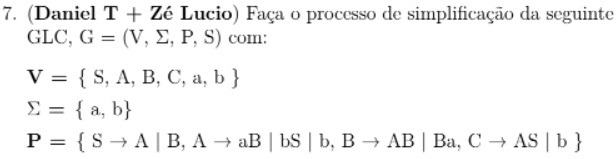
\includegraphics[width=15cm]{7.png} \\
    \caption{Processo de simplificação} \label{7}

  \end{center}
 \end{figure}
 \begin{figure}[h]
  \begin{center}
    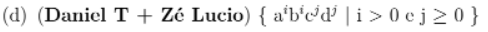
\includegraphics[width=15cm]{8.png} \\
    \caption{Projete GLC para a linguagem} \label{8}

  \end{center}
 \end{figure}
\section{Perguntas sobre Expressões Regulares}
 \begin{figure}[h]
  \begin{center}
    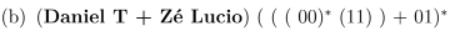
\includegraphics[width=15cm]{2.png} \\
    \caption{Converta E.R. em NFAs} \label{2}

  \end{center}
 \end{figure}
% ----------------------------------------------------------
% Capitulo com exemplos de comandos inseridos de arquivo externo
% ----------------------------------------------------------

\include{abntex2-modelo-include-comandos}


% ----------------------------------------------------------
% Parte de resultados
% ----------------------------------------------------------
\part{Resultados}
% ---
% Capitulo de revisão de literatura
% ---
\chapter{Apresentação dos resultados}
\section{Perguntas sobre GLC}
\begin{figure}[h]
  \begin{center}
    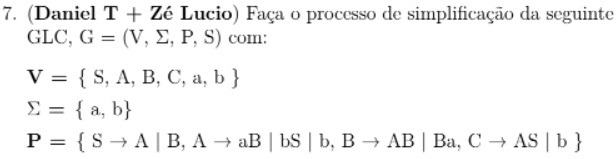
\includegraphics[width=15cm]{7.png} \\
    \caption{Processo de simplificação} \label{r7}

  \end{center}
 \end{figure}
 \begin{figure}[h]
  \begin{center}
    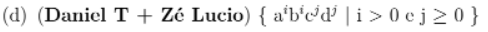
\includegraphics[width=15cm]{8.png} \\
    \caption{Projete GLC para a linguagem} \label{r8}

  \end{center}
 \end{figure}
\section{Perguntas sobre Expressões Regulares}
 \begin{figure}[h]
  \begin{center}
    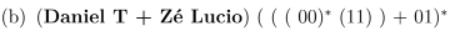
\includegraphics[width=15cm]{2.png} \\
    \caption{Converta E.R. em NFAs} \label{r2}

  \end{center}
 \end{figure}
% ---

\lipsum[1]

\lipsum[2-3]

% ---
% Finaliza a parte no bookmark do PDF
% para que se inicie o bookmark na raiz
% e adiciona espaço de parte no Sumário
% ---
\phantompart

% ---
% Conclusão
% ---
\chapter{Conclusão}
% ---

\lipsum[31-33]

% ----------------------------------------------------------
% ELEMENTOS PÓS-TEXTUAIS
% ----------------------------------------------------------
\postextual

% ----------------------------------------------------------
% Referências bibliográficas
% ----------------------------------------------------------
\bibliography{abntex2-modelo-references}

% ----------------------------------------------------------
% Glossário
% ----------------------------------------------------------
%
% Consulte o manual da classe abntex2 para orientações sobre o glossário.
%
%\glossary

% ----------------------------------------------------------
% Apêndices
% ----------------------------------------------------------
\begin{comment}
% ---
% Inicia os apêndices
% ---
\begin{apendicesenv}

% Imprime uma página indicando o início dos apêndices
\partapendices

% ----------------------------------------------------------
\chapter{Quisque libero justo}
% ----------------------------------------------------------

\lipsum[50]

% ----------------------------------------------------------
\chapter{Nullam elementum urna vel imperdiet sodales elit ipsum pharetra ligula
ac pretium ante justo a nulla curabitur tristique arcu eu metus}
% ----------------------------------------------------------
\lipsum[55-57]

\end{apendicesenv}
% ---


% ----------------------------------------------------------
% Anexos
% ----------------------------------------------------------

% ---
% Inicia os anexos
% ---
\begin{anexosenv}

% Imprime uma página indicando o início dos anexos
\partanexos

% ---
\chapter{Morbi ultrices rutrum lorem.}
% ---
\lipsum[30]

% ---
\chapter{Cras non urna sed feugiat cum sociis natoque penatibus et magnis dis
parturient montes nascetur ridiculus mus}
% ---

\lipsum[31]

% ---
\chapter{Fusce facilisis lacinia dui}
% ---

\lipsum[32]

\end{anexosenv}

%---------------------------------------------------------------------
% INDICE REMISSIVO
%---------------------------------------------------------------------

\phantompart

\printindex

%---------------------------------------------------------------------
% Formulário de Identificação (opcional)
%---------------------------------------------------------------------
\chapter*[Formulário de Identificação]{Formulário de Identificação}
\addcontentsline{toc}{chapter}{Exemplo de Formulário de Identificação}
\label{formulado-identificacao}

Exemplo de Formulário de Identificação, compatível com o Anexo A (informativo)
da ABNT NBR 10719:2015. Este formulário não é um anexo. Conforme definido na
norma, ele é o último elemento pós-textual e opcional do relatório.

\bigskip

\begin{tabular}{|p{9cm}|p{5cm}|}
\hline
\multicolumn{2}{|c|}{\textbf{\large Dados do Relatório Técnico e/ou científico}}\\
\hline
\multirow{4}{10cm}[24pt]{Título e subtítulo}& Classificação de segurança\\
                   & \\
                   \cline{2-2}
                   & No.\\
                   & \\

\hline
Tipo de relatório & Data\\
\hline
Título do projeto/programa/plano & No.\\
\hline
\multicolumn{2}{|l|}{Autor(es)} \\
\hline
\multicolumn{2}{|l|}{Instituição executora e endereço completo} \\
\hline
\multicolumn{2}{|l|}{Instituição patrocinadora e endereço completo} \\
\hline
\multicolumn{2}{|l|}{Resumo}\\[3cm]
\hline
\multicolumn{2}{|l|}{Palavras-chave/descritores}\\
\hline
\multicolumn{2}{|l|}{
Edição \hfill No. de páginas \hfill No. do volume \hfill Nº de classificação \phantom{XXXX}} \\
\hline
\multicolumn{2}{|l|}{
ISSN \hfill \hfill Tiragem \hfill Preço \phantom{XXXXXXXX}} \\
\hline
\multicolumn{2}{|l|}{Distribuidor} \\
\hline
\multicolumn{2}{|l|}{Observações/notas}\\[3cm]
\hline
\end{tabular}
\end{comment}
\end{document}
